\documentclass[11pt,a5paper]{article}
\usepackage{xcolor}
\usepackage[T1]{fontenc}
\usepackage[utf8]{inputenc}
\usepackage[greek, italian]{babel}
\usepackage{alltt}
\usepackage{scrextend}
\usepackage{geometry}
\usepackage[default]{opensans}
\usepackage{eso-pic}
\usepackage{tikz}
\usepackage{titlesec}
\usepackage[most]{tcolorbox}
\definecolor{block-gray}{gray}{0.82}
\newtcolorbox{myquote}{colback=block-gray,grow to right by=-10mm,grow to left by=-10mm, boxrule=0pt,boxsep=0pt,breakable}

\usepackage{titlesec}
\usepackage{graphicx}
\usepackage{transparent}
\usepackage{ifthen}
\usepackage{changepage}
\usepackage{fdsymbol}
\usepackage[final,kerning=true,spacing=true,tracking=true,activate={true,nocompatibility},stretch=10,shrink=10]{microtype}

\usepackage{tabularx}
\usepackage{tabto}
\usepackage{setspace}
\usepackage{tocloft}

\SetTracking{encoding={*}, shape=sc}{0}
\SetExtraKerning[unit=space]{encoding=T1}{'={160,280},”={250,0},“={0,100}}

\newlength{\sectionnumlen}
\setlength{\sectionnumlen}{30pt}

\titleformat{\section}%
{\fontfamily{ppl}\selectfont\fontsize{16}{24}\selectfont\scshape\bfseries}%
{\makebox[\sectionnumlen][l]{\bfseries\scshape\thesection}}%
{0mm}%
{}%
[\vskip -0.1cm plus 0.1cm minus 0.1cm]%

% Per aggiungere il logo SNS in trasparenza ad alcune pagine
\newif\iflogo
\AddToShipoutPictureBG{
  \iflogo{%
    \put(280,390){%
      \transparent{0.17}
\includegraphics[width=3.5cm]{images/logo_SNS_nero}%
    }%
  }\else\fi%
}

\newcommand{\RIT}{%
  \vspace*{-0.3em}%
  {~\hfill{\fontfamily{ppl}\selectfont $\vardiamondsuit${\hskip 0.5em}RIT.{\hskip 0.5em}$\vardiamondsuit$}\hfill~}%
  \vspace*{-0.3em}%
}

\newcommand{\ARIT}{%
  {\fontfamily{ppl}\selectfont RIT.}%
}

\newcommand{\RITB}{%
  \vspace*{-0.3em}%
  {~\hfill{\fontfamily{ppl}\selectfont $\vardiamondsuit${\hskip 0.5em}RIT. x2{\hskip 0.5em}$\vardiamondsuit$}\hfill~}%
  \vspace*{-0.3em}%
}

\newcommand{\ALLREP}[1]{%
	{\fontfamily{ppl}\selectfont {\hskip 0.5em}(Tutto x#1){\hskip 0.5em}}%
}

\makeatletter
\renewcommand{\@seccntformat}[1]{%
  \begingroup
  \@nameuse{additional@cntformat#1}%
  {\@nameuse{the#1}}%
  \endgroup
  \quad
}
\newcommand{\setformat}[2]{%
  \@namedef{additional@cntformat#1}{#2}%
}
\makeatother

% \setformat{section}{\LARGE}

\definecolor{ourgray}{HTML}{606060}
\newcommand{\santanna}{{\normalsize s}ant'{\normalsize a}nna}
\newcommand{\subtitle}[1]{\vspace*{-0.7em}%
  {\makebox[\sectionnumlen][l]{}\textcolor{ourgray}{\fontsize{11.5}{16}\selectfont\it #1}}}
\renewcommand{\title}[1]{%
  \begin{center}%
    {\fontfamily{pag}\selectfont\scshape\Huge{#1}}%
  \end{center}%
}

\newlength{\aritlen}
\settowidth{\aritlen}{\ARIT: }

\newcommand{\aritskip}{\makebox[\aritlen][l]{}}

\newenvironment{canzone}{%
  \begin{adjustwidth}{\sectionnumlen}{}%
  \begin{alltt}\normalfont%
  }{%
  \end{alltt}%
  \end{adjustwidth}%
}

\begin{document}
\logofalse
\newgeometry{top=0mm,bottom=0mm,left=0mm,right=0mm}
\fontsize{13}{16}\selectfont
\setlength{\parindent}{0cm}
\setlength{\parskip}{1.0em plus 0.4em minus 0.2em}
\linespread{1.25}
\pagestyle{empty}

%% -- PRIMA DI COPERTINA
\leavevmode
\put(50,70){
  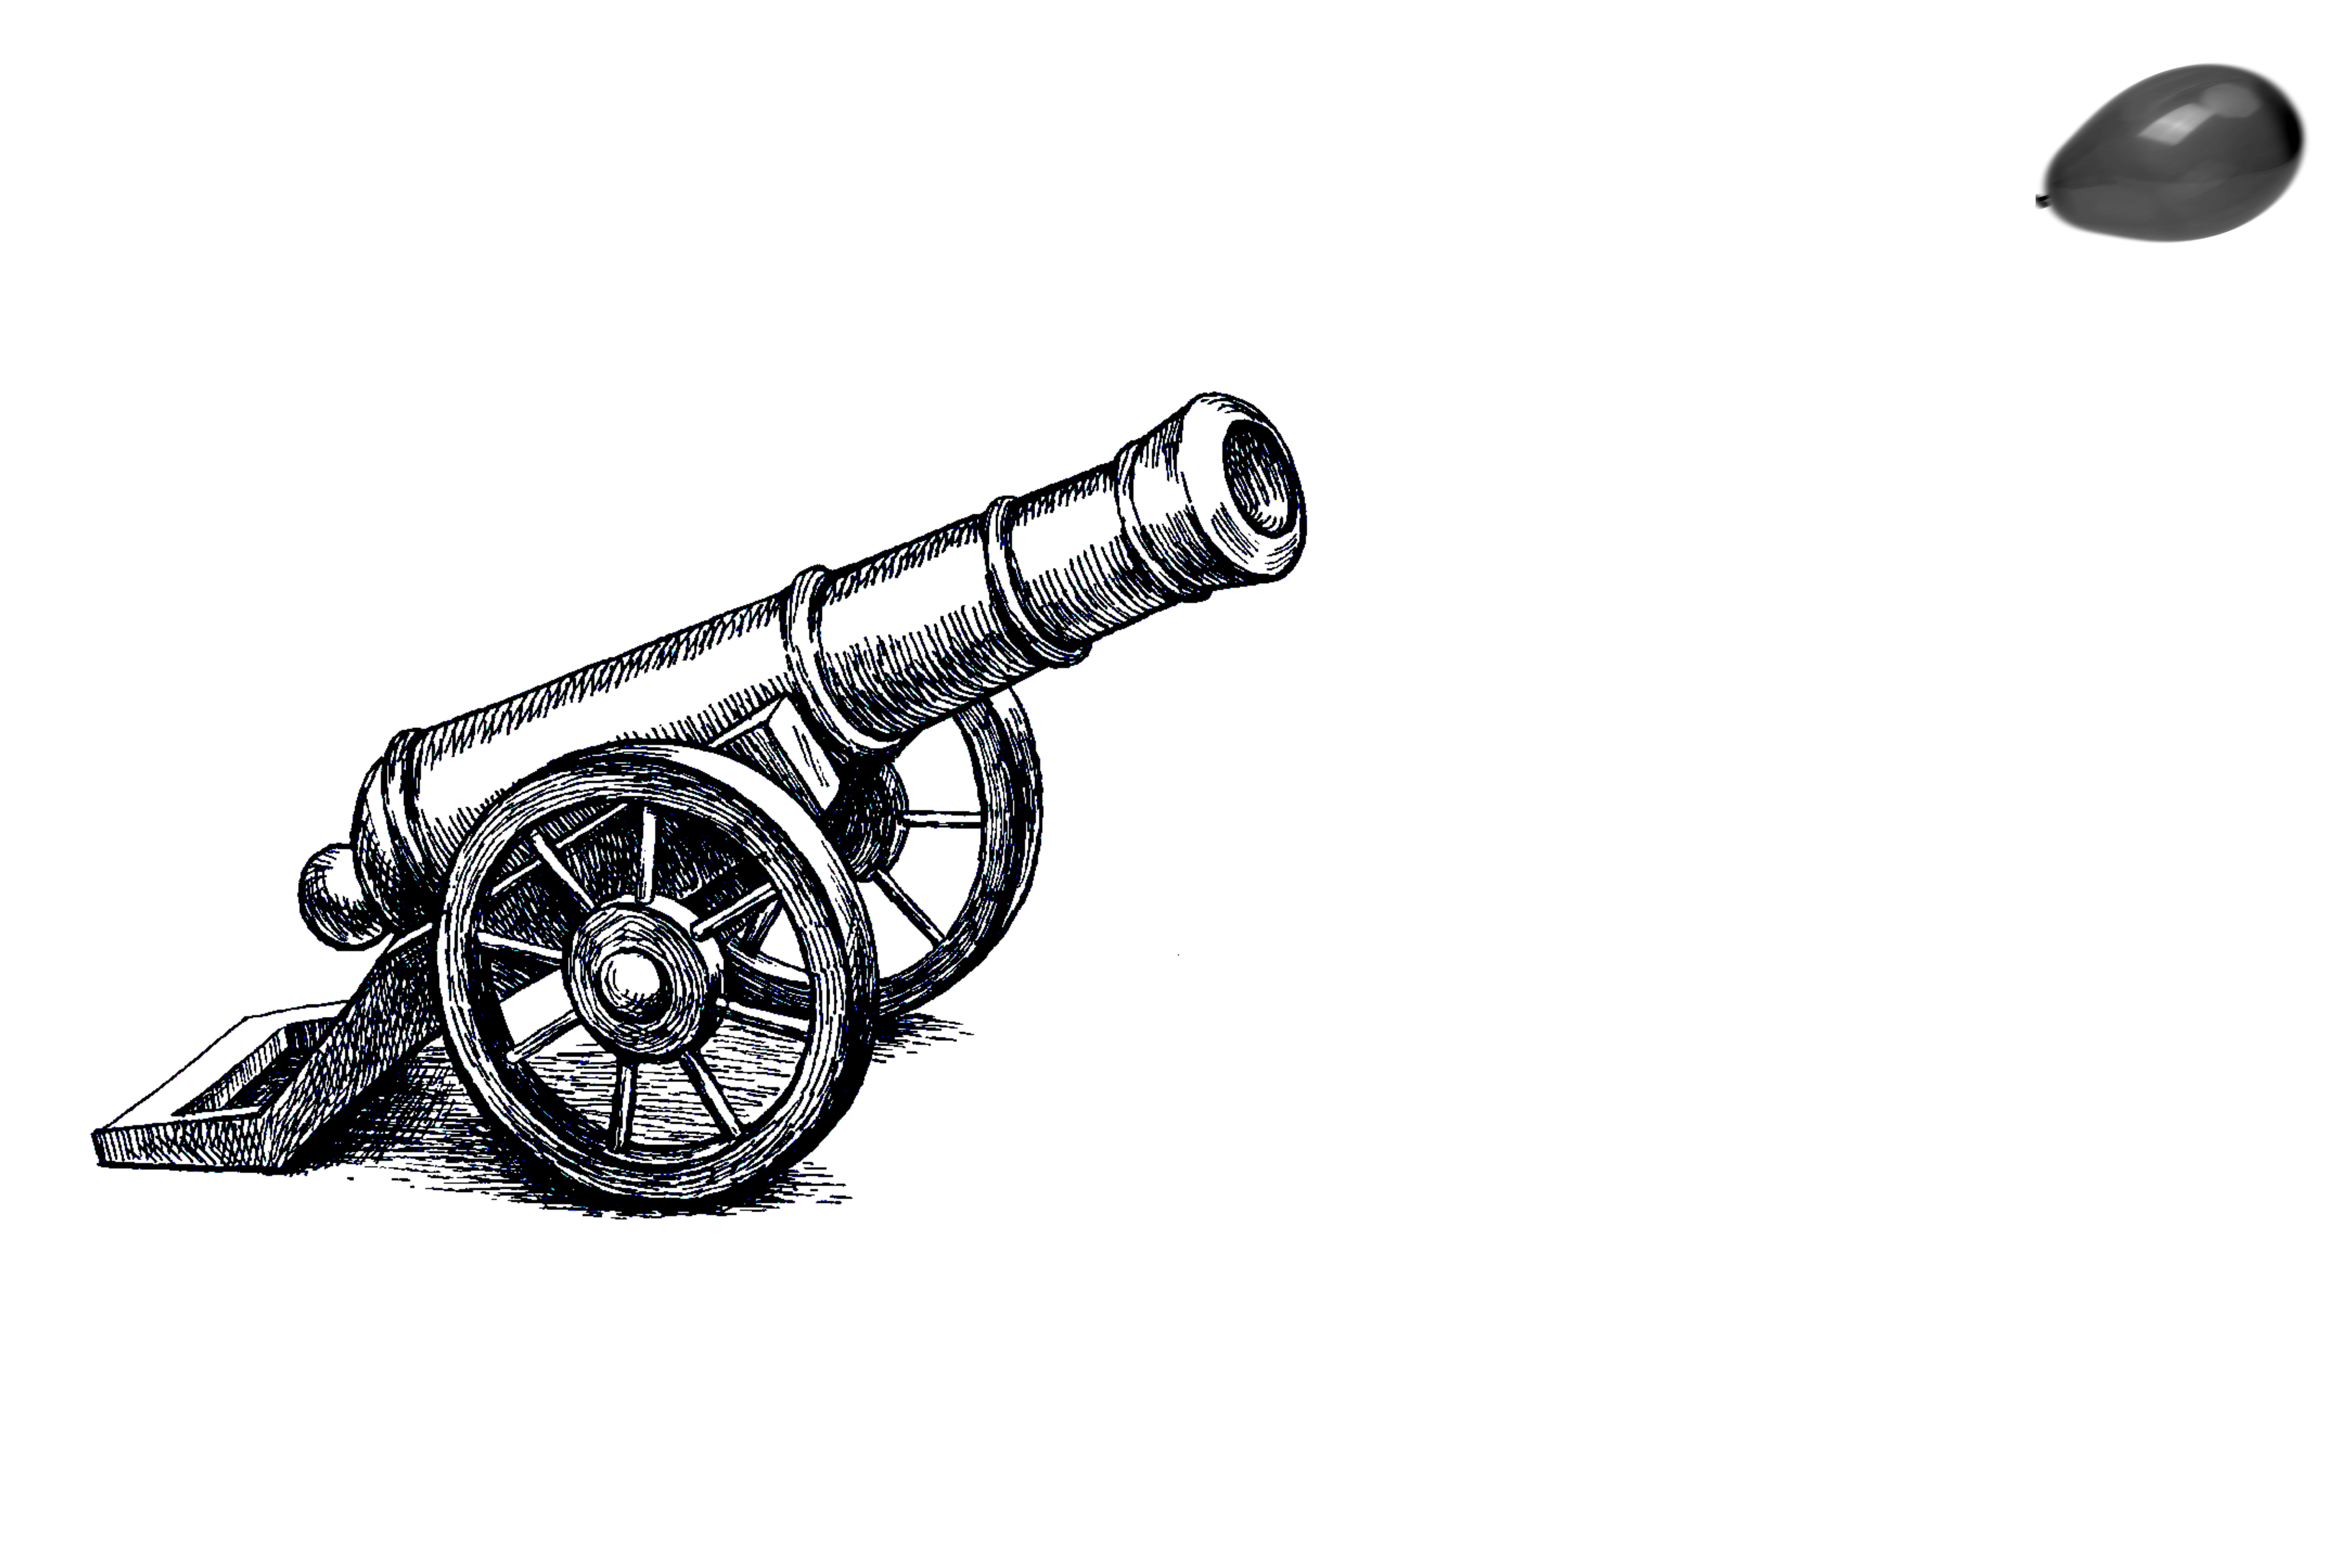
\includegraphics[width=0.70\textwidth]{images/miniatura}
}
\leavevmode
\put(-3,-1){
  
\includegraphics[width=\dimexpr\textwidth\relax,height=\dimexpr\textheight-0.05mm\relax]{images/cornice}
}
\leavevmode
\put(60,300){
  
\includegraphics[width=0.70\textwidth]{images/striscione}
}
\clearpage


\if twoside
\newgeometry{top=20mm,inner=20mm,outer=10mm,bottom=20mm}
\else
\newgeometry{top=20mm,left=15mm,right=15mm,bottom=20mm}
\fi
%% -- CITAZIONE E RINGRAZIAMENTI
\begin{myquote}\it
  Chi vince la guerra scrive la storia,\\
  chi perde la guerra scrive i giornali.
  
  {~\hfill\normalfont -- Francesco Guatieri}
\end{myquote}

\vfill

\begin{adjustwidth}{\sectionnumlen}{}\fontsize{10}{15}\selectfont
  Cornice e Titolo di Marta Tasinato\\
  Adeguamento Immagini di Piero Lafiosca ed Enrico Polesel\\
  Correzione testi di Nicolò Campodonico\\
  Impaginazione e Layout di Dario Balboni
\end{adjustwidth}
\clearpage


\logotrue
%% -- INIZIO DEL CANZONIERE
\title{Canzoniere di Guerra}
\title{della}
\title{Scuola Normale Superiore}
\begin{center}%
	{\fontfamily{pag}\selectfont\scshape\Large{(Versione CD)}}%
\end{center}%

\clearpage
\section{Alla Normale urrà!}
\subtitle{Sulla melodia di “When Johnny comes marching home”}
\begin{canzone}
È pronta la Normale per le avversità:
Abbiam giurato tutti non aver pietà!
I gavettoni alla fanteria,
Dalle finestre l’artiglieria,
Fremono gli idranti.
Per la Normale urrà!

Non hanno i santannini alcuna dignità:
Son tutti dei fascisti figli di papà;
Non hanno fatto neanche un bidet
Sin dal lontano sessantatré:
È arrivato il puzzo
Sino in Normale già!

Vedendoli fuggire ed implorar pietà,
Mostriamo ai loro anziani cos’è l’umiltà
E da sevizie ridicole
Salviam le loro matricole,
Che dovran la vita
Alla Normale, urrà! 

E da sevizie ridicole
Salviam le loro matricole,
Che dovran la vita
Alla Normale, urrà! (x2)
\end{canzone}

\section{Scuola Normale la trionferà}
\begin{canzone}
Puzza di fogna, ti attacca il tifo,
pidocchi e rogna, fa proprio schifo!
È il santannino, è un animale,
ma la Normale lo domerà.

Scuola Normale la trionferà!
Scuola Normale la trionferà
e il santannino che la sfiderà
lavato con Perlana si ritirerà!

Noi integriamo gli operatori,
campi finiti, quadritensori;
mentre al \santanna - che gran buffoni! - 
solo addizioni sapete far.

Scuola Normale la trionferà!
Scuola Normale la trionferà
e il santannino che la sfiderà
lavato con Perlana si ritirerà!

\clearpage
I santannini sono ingegneri,
sono giuristi, son parrucchieri.
Ma quale genio? Ma che eccellenza?
La vera scienza si fa in Normal!

Scuola Normale la trionferà!
Scuola Normale la trionferà!
Scuola Normale la trionferà!
Se liberiam Barbieri chi vi salverà?
\end{canzone}

\vspace{0.6in}
\section{Son perdenti, son sfigati}
\subtitle{Sul canto tipico dei marines}

\subtitle{Ogni verso si canta due volte}
\begin{canzone}
Son perdenti, son sfigati
I giuristi e gli avvocati!
Gli ingegneri, che buffoni:
Sbaglian pure le addizioni!

Destinato è il santannino
Solo a fare lo spazzino!
Canta in cor la nostra truppa:
S.S.S.U.Puppa!
\end{canzone}

\clearpage
\section{Nella notte più nera}
\subtitle{Sulla melodia di “Let's Go“ del Coro dell’Armata Rossa}
\begin{canzone}
Nella notte più nera
Non cerchiamo il sole, mio signor!
Ma solo uno scudo e uno stemma bianco e blu
Che ci porti ancor più su, 
Ancor più su,
Su, su!
Uniti contro il male,
Lottiam per la Normale:
La vittoria cerchiam e arriverà!

Noi di folgore non armati
I cieli squarceremo, sì!
Ché di gavettoni tempesta sorgerà
Che affondi il Sant’Anna giù, 
Ancor più giù, 
Giù, giù!
Nell’abisso più infame,
Più delle loro brame
Di aver la dignità
Della Normal!

Come fiera testuggine
L’oscuro mare fermerem
E quando la luce infine tornerà
L’onda azzurra crescerà,
L’abbatterà 
Là, là!
Là nelle loro tane
Di sevizie inumane.
La Storia canterà:
Normale urrà!
\end{canzone}

\vspace{0.6in}
\section{Sono gli scemi del \santanna}
\subtitle{Ogni verso si canta due volte}
\begin{canzone}
Ovunque voi andiate,
Noi ci siamo.
La genta ci domanda:
“Ma chi sono?”
Sono gli scemi del Sant’Anna,
Tutti segati alla Normale,
Che per cercar di rimediare
Vanno a far finta di studiare. 
\end{canzone}

\clearpage
\section{L’han segato alla Normal}
\begin{canzone}
Come un animale, si sveglia ogni mattino,
avviterà bulloni, è infelice il santannino.
Voleva esser fisico, studiare la natura,
ma della sua ignoranza sì che c'è da aver paura.

\aritskip L’han segato alla Normal!
\aritskip Segato resterà
\aritskip e con gli altri segati
\aritskip lui è andato a star.

D'estate una mattina lui è andato all'ammissione,
credeva d'esser genio, ma era solo un gran coglione.
Di fronte a quei problemi non sapeva cosa fare:
almeno le addizioni eran cosa da imparare.

\RIT

Qualche giorno dopo in Santa Caterina
gli chiedon se è capace di avvitar la lampadina.
Lui prova a caso un verso, credendo sia lo stesso,
al terzo tentativo finalmente viene ammesso.

\RIT

Da povera matricola, quand'era appena entrato,
com'essere inferiore lui è stato seviziato.
Onora i suoi anziani ritenendoli speciali,
non sa d'esser finito dentro a un covo di animali.

\RIT

Solo tre anni dopo devon scriver le tesine:
chiodi, viti oppure scienza delle merendine?
Anche laureato lui continua a rosicare
perché da un Normalista avrebbe solo da imparare.

\RIT

Giunto al quinto anno la sua essenza ha rivelato:
pelliccia attorno al corpo e cervello obnubilato.
Il suo pensiero fisso lo tormenta ogni ora.
Quella bocciatura, mamma mia se brucia ancora!

\RITB
\end{canzone}

\clearpage
\section{Il ponte sul fiume Arno}
\subtitle{Su “Colonel Bogey March” dal film “Il ponte sul fiume Kwai”}
\begin{canzone}
Guarda, che cosa vedi là?
Sembra il culo d’un maial
E invece è un santannino,
Steccò persino il test in Normal!

Puzza come un animal,
Studia, ma resta un gran somar.
Merda di un santannino,
Fatti vicino: ti devo lavar!
\end{canzone}

\vspace{1.2in}
\section{Il santannino puzza}
\subtitle{Sulla melodia della “Virginia Company”}
\begin{canzone}
Il santannino puzza,
Ma lo laveremo noi.
Se pure voi barate,
Non ci arrenderemo mai!
Con Vasco condottiero
E Beltram nostro dio,
Nostro sarà il trionfo
E voi cadrete nell’oblio!
Nostro sarà il trionfo
E voi cadrete nell’oblio!

Il normalista è fiero:
Non prova mai timor;
Combatte per dar gloria
Alla Normale Superior.
E abbiamo dalla nostra
Anche la gravità,
Se un giorno mai scopriste
Che anche l’acqua in basso va:
Ma siete troppo scemi
E la Normale vincerà!
\end{canzone}

\clearpage
\section{Ma al \santanna\ no}
\subtitle{Sulla melodia di “Ma la notte no”}
\begin{canzone}
Quasi tutta la gente ha un’igiene decente,
Ma al Sant'Anna no!

Relazioni normali ci son tra gli animali,
Ma al Sant'Anna no!

Moderarsi ai processi lo san fare anche i fessi,
Ma al Sant'Anna no!

Quasi ovunque in natura si è trovata una cura,
Ma al Sant'Anna no!

Disegnare una theta lo fa un analfabeta,
Ma al Sant'Anna no!

Cosa son le equazioni lo san pure i coglioni,
Ma al Sant'Anna no!

Quattro conti azzeccati li fan pure i primati,
Ma al Sant'Anna no!

L’intuizione geniale sempre abbonda in Normale,
Ma al Sant'Anna no!

Urrà, urrà, urrà alla Normale,
Ma al Sant'Anna no! 
(si ripete quattro volte)
\end{canzone}

\clearpage
\section{Il sogno alla Normale}
\subtitle{Sulla melodia di “Il sogno di un Pisano”}
\begin{canzone}
Il sogno alla Normale è 
Svegliarsi la mattina
E veder bruciare 
Piazza Santa Caterina! 
\end{canzone}

\section{Sis triumphans, o Schola Normalis}
\begin{canzone}
Sis triumphans, o Schola Normalis,
mundi splendor, spes nostrae salutis. \hspace{2em} {\small x2}
Summae norma tu vere virtutis,
artis, linguae et scientiae studiosa. \hspace{3.4em} {\small x2}

{\normalsize s}anctae {\normalsize a}nnae sic bestia domata,
triumphatrix sis scientiae regina. \hspace{4.2em} {\small x2}
Et placata sua ira divina,
Normalista nunc studet in pace. \hspace{4.5em} {\small x2}

Vivat! Vivat! Vivat Normalis! \hspace{6.8em} {\small x2}
\end{canzone}

\section{Priore ciao}
\subtitle{Sulla melodia di “Bella ciao“}
\begin{canzone}
Una mattina mi son svegliato,
O priore ciao, priore ciao, priore ciao, ciao, ciao!
Una mattina mi son svegliato,
E ho trovato il santannin.

O normalista, portami via!
O priore ciao, priore ciao, priore ciao, ciao, ciao!
O normalista, portami via:
Questo puzza da morir!

E se io muoio con il mio scudo,
O priore ciao, priore ciao, priore ciao, ciao, ciao!
E se io muoio con il mio scudo,
Tu mi devi seppellir.

E seppellire là in Carovana,
O priore ciao, priore ciao, priore ciao, ciao, ciao!
E seppellire là in Carovana,
Sotto l’ombra di Beltram.

Tutti i pisani che passeranno,
O priore ciao, priore ciao, priore ciao, ciao, ciao!
Tutti i pisani che passeranno,
Mi offriranno un gavetton.

Questa è la bomba del normalista,
O priore ciao, priore ciao, priore ciao, ciao, ciao!
Questa è la bomba del normalista
Morto con lo scudo in man.
\end{canzone}

\clearpage
\section{L'Arno mormorava}
{\setstretch{1.2}\fontsize{13}{16}\selectfont
\begin{canzone}
L'Arno mormorava
calmo e placido di fronte
ai primi allievi in marcia sopra il ponte.
L'esercito avanzava,
trasportava i propri scudi,
mostrando al vento i fieri petti ignudi.

Carrelli ovunque pien di gavettoni!
Andavano a lavar quei gran puzzoni!

S'udiva intanto dalle vie d'intorno
il forte canto ed il suonar del corno.
Era il gran grido delle invitte schiere.

E l'Arno mormorò:
"Non passa l'ingegnere!"

Ma dopo la battaglia
si parlò di codardia,
ch'era il nemico presto corso via.
Saliva la marmaglia
sulle scale in Cavalieri,
dava una foto in pasto a dei ciarlieri.

Giornali scrive certo non la storia
il santannino che grida vittoria.

Veniva intanto in mente a ogni buffone
il tempo dell'esame d'ammissione.
Credeva d'esser genio di sapere.

Ma il test comandò:
"Segato è l'ingegnere!"

E ritornò una sera
in San Francesco la tenzone:
si miser tutti quanti in formazione.
S'ergeva tra la schiera
maestoso un gran fortino:
sottrasse ogni speranza al santannino!

Carrelli, ultrà e scudi ancor più grossi
e il fuoco e i calici scottanti e rossi!

Cercò la feccia allor di rimediare
Le scale in Carovana di occupare
Ma i Normalisti eran lì a tenere.

La piazza comandò:
"Indietro va', ingegnere!"

E indietreggiò sconfitto
fino in Santa Caterina,
si chiuse nella sua volgar latrina.
Placatosi il conflitto
tra le schiere il Costruttore
apparve assieme al nostro Gran Priore!

Sancì allora questa sacra vista
la nobile vittoria normalista!

Sicura casa e libere le scale
e tacque l'Arno e si zittì il giornale.
Sul patrio suolo vinti gl'ingegneri,

la scienza non trovò
spazzini e parrucchieri!
\end{canzone}
}

\clearpage
\section{Santannin}
\begin{canzone}
Dalla piazza Cavalieri,
sotto l'acqua santannina,
se ne infischiano del gelo
gli studenti alla Normal.

Col Fortino e i frombolieri,
camminando tutti in fila,
con lo scudo saldo in mano
vanno contro il santannin.

Santannin,
studi, studi e dopo un po'
corri pronto a vomitare
le nozioni al professor.
Santannin,
in battaglia che cos'hai?
Rubi i fondi della scuola
ma non possono bastar.

\clearpage
I normalisti lunghi e fieri,
con gli scudi volti in su,
i gavettoni san tirare
e il santannino non c'è più.

È rimasto senza fiato
sulla pancia accovacciato.
Che istituto sfortunato
S.S.S.U.P.!

Santannin,
studi, studi e dopo un po'
...

Dietro al pubblico pisano,
prima dell'ultimo round,
c'é una truppa d'eccezione:
è la squadra di Beltram.

Mentre i nostri in formazione
fanno fuoco per l'onor,
loro vanno in Carovana
a difender lo scalon.

Santannin,
corri, corri e arriverai
solo contro mille scudi
che ti forzano a scappar.
Santannin,
ma l'assalto dove sta?
Ci son solo quattro scemi
ma non possono bastar!
\end{canzone}

\vspace{1in}
\section{Il vero Normalista}
\begin{canzone}
Rischia il freddo il vero Normalista;
cinque esami, eppur bisogna andar
a conquistar piazza Santa Caterina,
dove sorge il covo santannin.
A conquistar piazza Santa Caterina,
dove sorge il covo santannin.

\clearpage
Ogni collegio è pieno di fervore,
ogni soldato brama di lavar.
Nella notte lo guida il Gran Priore,
forte il cuore e il braccio nel lanciar.
Nella notte lo guida il Gran Priore,
forte il cuore e il braccio nel lanciar.

Se ci coglie in testa un gavettone,
dura vendetta sarà della Normal.
Ormai sicura è la sorte del buffone
santannino vile traditor.
Ormai sicura è la sorte del buffone
santannino vile traditor.

Cessa il fuoco, lo scudo si riposa,
torna a casa fiera la Normal,
celebrando l'armata più gloriosa,
vittoriosi alfin asciutti siam!
Celebrando l'armata più gloriosa,
vittoriosi alfin asciutti siam!
Celebrando l'armata più gloriosa
vittoriosi alfin asciutti siam!
\end{canzone}

\clearpage
\logofalse
\newgeometry{top=0mm,bottom=0mm,left=0mm,right=0mm}
%% -- ULTIMA DI COPERTINA
\leavevmode
\put(55,125){
  {\transparent{0.8}\includegraphics[width=0.70\textwidth]{images/fregio}}
}
\leavevmode
\put(0,0){
  
\includegraphics[width=0.96\textwidth]{images/cornice}
}


\end{document}

